%% Template for a preprint Letter or Article for submission
%% to the journal Nature.
%%

\documentclass[%
%superscriptaddress,
%groupedaddress,
%unsortedaddress,
%runinaddress,
%frontmatterverbose, 
%preprint,
showpacs,
%preprintnumbers,
nofootinbib,
%nobibnotes,
%bibnotes,
 amsmath,amssymb,
 aps,
 twocolumn,
 prl,
 reprint,
%pra,
%prb,
%rmp,
%prstab,
%prstper,
floatfix,
]{revtex4-1}

\usepackage{graphicx}% Include figure files
\usepackage{dcolumn}% Align table columns on decimal point
\usepackage{bm}% bold math
%\usepackage{lineno}
\usepackage{amsmath}
\usepackage{amsfonts}
\usepackage{amssymb}
\usepackage{color}
\usepackage{acronym}
\usepackage{multirow}
\usepackage{tabularx}
\usepackage{hyperref}
\usepackage{mathtools}
%\usepackage{booktabs}

\hypersetup{
%--- fill inside borders ---
  colorlinks=true,        % false: boxed links; true: colored links
  linkcolor=black,         % color of internal links
  citecolor=cyan,         % color of links to bibliography
}

%% ----- comment commands for each of us
\newcommand{\chris}[1]{\textbf{\textcolor{red}{CHRIS: #1}}}
\newcommand{\francesco}[1]{\textbf{\textcolor{green}{FRANCESCO: #1}}}
\newcommand{\hunter}[1]{\textbf{\textcolor{blue}{HUNTER: #1}}}
\newcommand{\siong}[1]{\textbf{\textcolor{cyan}{SIONG: #1}}}
\newcommand{\rod}[1]{\textbf{\textcolor{yellow}{ROD: #1}}}
\newcommand{\new}[1]{\textcolor{red}{#1}}

\begin{document}

\preprint{APS/123-QED}

\title{Bayesian parameter estimation using conditional variational autoencoders
for gravitational-wave astronomy}

\author{Hunter Gabbard$^1$}
 \email{Corresponding author: h.gabbard.1@research.gla.ac.uk}
\author{Chris Messenger$^1$}
\author{Ik Siong Heng$^1$}
\author{Francesco Tonolini$^2$}
\author{Roderick Murray-Smith$^2$}

\affiliation{
 SUPA, School of Physics and Astronomy$^1$, \\
 University of Glasgow, \\
 Glasgow G12 8QQ, United Kingdom \\ \\
 School of Computing Science$^2$, \\
 University of Glasgow, \\
 Glasgow G12 8QQ, United Kingdom \\
}

\date{\today}

\maketitle

% TO-DO LIST
%
% 1. Get abstract word count roughly correct - currently 195 (done)
% 2. Get total word count roughly correct - currently (195, 680, 960, 620) =
% 2455
% 3. Clean captions and check word count (done)
% 4. Fix all plots (done)
% 5. Tidy Methods section (done)
% 6. Polish language throughout (done)
% 7. Check acronyms for consistency
% 8. Check names and variables for consistency (KL, VItamin, etc...)
% 9. Fix references - check limit
% 10. Maybe change title
% 11. Maybe add extra plots to methods section
% 12. Do a spell check (done)
% 13. Fix acknowledgments (done)
% 14. Clean codes and add ref to github

\acrodef{GW}[GW]{Gravitational wave}
\acrodef{BBH}[BBH]{binary black hole}
\acrodef{EM}[EM]{electromagnetic}
\acrodef{CBC}[CBC]{compact binary coalescence}
\acrodef{BNS}[BNS]{binary neutron star}
\acrodef{NSBH}[NSBH]{neutron star black hole}
\acrodef{PSD}[PSD]{power spectral density}
\acrodef{ELBO}[ELBO]{evidence lower bound}
\acrodef{LIGO}[LIGO]{advanced Laser Interferometer Gravitational wave Observatory}
\acrodef{CVAE}[CVAE]{conditional variational autoencoder}
\acrodef{KL}[KL]{Kullback--Leibler}
\acrodef{GPU}[GPU]{graphics processing unit}
\acrodef{LVC}[LVC]{LIGO-Virgo Collaboration}
\acrodef{PP}[p-p]{probability-probability}

%
% Introductory paragraph describing the content of the letter
%
% This format begins with a title of, at most, 15 words, followed by an
% introductory paragraph (not abstract) of approximately 150 words, summarizing
% the background, rationale, main results (introduced by "Here we show" or some
% equivalent phrase) and implications of the study. This paragraph should be
% referenced, as in Nature style, and should be considered part of the main
% text, so that any subsequent introductory material avoids too much redundancy
% with the introductory paragraph.
%
\textbf{ 
%
% background
%
\ac{GW} detection is now
commonplace~\cite{PhysRevX.6.041015,PhysRevLett.119.161101} and as the
sensitivity of the global network of \ac{GW} detectors improves, we will
observe $\mathcal{O}(100)$s of transient \ac{GW} events per
year~\cite{2018LRR....21....3A}. The current methods used to estimate their
source parameters employ optimally sensitive~\cite{2009CQGra..26o5017S} but
computationally costly Bayesian inference approaches~\cite{1409.7215} where
typical analyses have taken between 6 hours and 5 days~\cite{gracedb_O3}.
%
% rationale
%
For \ac{BNS} and \ac{NSBH} systems prompt counterpart \ac{EM} signatures are
expected on timescales of 1 second -- 1 minute and the current fastest method
for alerting \ac{EM} follow-up observers~\cite{2016PhRvD..93b4013S}, can
provide estimates in $\mathcal{O}(1)$ minute, on a limited range of key source
parameters. 
%
% results
%
Here we show that a \ac{CVAE}~\cite{1904.06264,1812.04405} pre-trained on
\ac{BBH} signals can return Bayesian posterior probability estimates. The
training procedure need only be performed once for a given prior parameter
space and the resulting trained machine can then generate samples describing
the posterior distribution $\sim 6$ orders of magnitude faster than existing
techniques.}
%
% currently ~240 words - needs cutting to ~150 approx 9.6 words per line

%%%%%%%%%%%%%%%%%%%%%%%%%%%%%%%%%%%%%%%%%%%%%%%%%%%%%%%%%%%%%%%%%%%%%%
% INTRODUCTION
%%%%%%%%%%%%%%%%%%%%%%%%%%%%%%%%%%%%%%%%%%%%%%%%%%%%%%%%%%%%%%%%%%%%%%
%
% introduction - this section has to expand upon what has mentioned in the
% abstract background (which was only ~50 words). It needs to cover the state of
% the gravitational wave field and the number of detections expected in the next
% ~5 years. It should briefly discuss the issue of low latency EM follow up. It
% needs to cover Bayesian inference (not in too much detail) and the signal model
% we are interested in here (again, not too much detail but enough for the
% average Nature reader). It then needs to introduce machine learning and focus
% mainly on how our scheme works. We also need to include a statement about how
% the training data priors affect the result (are they really the priors?)
%
% Intro to the detection era with the LVC
%
%With the overwhelmingly successful observation runs of O1 and O2 now complete,
%\ac{LIGO} and Virgo have produced a large catalogue of \ac{GW} data covering
%both \ac{BBH} and \ac{BNS} signals~\cite{1811.12907}. Over the next five years
%we expect the number of detections to increase to be upwards of $\sim180$
%\ac{BNS} and $\sim400$ BBH events per year~\cite{1304.0670,1811.12907}. This
%large influx in the number of detections will put an increased amount of
%pressure on the current \ac{GW} inference methods used for parameter
%estimation.  

%
% From GW detection, to parameter estimation
%
The problem of detecting \acp{GW} has largely been solved through the use of
template based matched-filtering, a process recently replicated using machine
learning techniques~\cite{GEORGE201864,PhysRevLett.120.141103,GebKilParHarSch}.
Once a \ac{GW} has been identified through this process, Bayesian inference,
known to be the optimal approach~\cite{2009CQGra..26o5017S}, is used to extract
information about the source parameters of the detected \ac{GW} signal.

%
% Set up parameter estimation problem
%
In the standard Bayesian \ac{GW} inference approach, we assume a signal and
noise model and both may have unknown parameters that we are either interested
in inferring or prefer to marginalise away. Each parameter is given a prior
astrophysically motivated probability distribution and in the \ac{GW} case, we
typically assume a Gaussian additive noise model (in reality, the data is not
truly Gaussian). Given a noisy \ac{GW} waveform, we would like to find an
optimal procedure for inferring some set of the unknown \ac{GW} parameters.
Such a procedure should be able to give us an accurate estimate of the
parameters of our observed signal, whilst accounting for the uncertainty
arising from the noise in the data.

%
% Describe Bayes Theorem
%
According to Bayes' Theorem, a posterior probability distribution on a set of
parameters, conditional on the measured data, can be represented as
%
\begin{align}\label{eq:bayes_theorem} 
p(x|y) &\propto p(y|x) p(x), 
\end{align}
%
where $x$ are the parameters, $y$ is the observed data, $p(x|y)$ is the
posterior, $p(y|x)$ is the likelihood, and $p(x)$ is the prior on the
parameters. The constant of proportionality, which we omit here, is
$p(y)$, the probability of our data, known as the Bayesian evidence or the
marginal likelihood. We typically ignore $p(y)$ since it is a constant and for
parameter estimation purposes we are only interested in the shape of the
posterior.

%
% brief statement on the sampling algorithms
%
Due to the size of the parameter space typically encountered in \ac{GW}
parameter estimation and the volume of data analysed, we must stochastically
sample the parameter space in order to estimate the posterior.  Sampling is
done using a variety of techniques including Nested
Sampling~\cite{skilling2006,cpnest,dynesty} and Markov chain Monte Carlo
methods~\cite{emcee,ptemcee}. The primary software tools used by the \ac{LIGO}
parameter estimation analysis are \texttt{LALInference} and
\texttt{Bilby}~\cite{1409.7215,1811.02042}, which offer multiple sampling
methods.  
  
%
% Intro to machine learning section
%
Machine learning has featured prominently in many areas of \ac{GW} research
over the last few years. These techniques have shown to be particularly
promising in signal
detection~\cite{GEORGE201864,PhysRevLett.120.141103,GebKilParHarSch}, glitch
classification~\cite{0264-9381-34-6-064003} and earthquake
prediction~\cite{Coughlin_2017}. We also highlight \new{recent developments in
\ac{GW} parameter estimation (independent to this work) where 1- and
2-dimensional marginalised Bayesian posteriors are produced rapidly using
neural networks~\cite{2019arXiv190905966C}, and where normalised flows in
conjunction with \acp{CVAE} can reproduce Bayesian posteriors for a single
\ac{GW} detector case~\cite{2020arXiv200207656G}. These methods, including the
one presented in this paper, are known as "likelihood-free" approaches in which
there is no requirement for explicit likelihood evaluation. Nor is it the case
that pre-computed posterior distributions are required in the training
procedure.}

%
% Introduce CVAEs
%
Recently, a type of neural network known as \ac{CVAE} was shown to perform
exceptionally well when applied towards computational imaging
inference~\cite{1904.06264,NIPS2015_5775}, text to image
inference~\cite{1512.00570}, high-resolution synthetic image
generation~\cite{1612.00005} and the fitting of incomplete heterogeneous
data~\cite{1807.03653}. It is this type of machine learning network that we
apply in the \ac{GW} case to accurately approximate the Bayesian posterior
$p(x|y)$, \new{the probability of the \ac{GW} signal parameters given the
measured data.} 

%
% Brief introduction to loss functions used in the neural networks
%
The construction of a \ac{CVAE} begins with the definition of a quantity to be
minimised (referred to as a cost function). \new{In our case we use the cross
entropy}, defined as
%
\begin{align}\label{eq:cross_ent} 
H(p,r) &= -\int dx\, p(x|y) \log r_{\theta}(x|y) 
\end{align}
%
between the true posterior $p(x|y)$ and $r_{\theta}(x|y)$, the parametric
distribution that we will use neural networks to \new{model} and which we aim
to be equal to the true posterior. \new{The parametric model is constructed from a
combination of 2 (encoder and decoder) neural networks $r_{\theta_1}(z|y)$ and
$r_{\theta_2}(x|y,z)$ where
%
\begin{align}\label{eq:latent_model}
r_{\theta}(x|y) = \int dz\,r_{\theta_1}(z|y)r_{\theta_2}(x|y,z).
\end{align}
%
In this case the $\theta$ subscripts represent sets of trainable neural
network parameters and the variable $z$ represents locations within a
\emph{latent space}. This latter object is typically a lower dimensional space
within which encoder networks attempt to represent their input data.}

Starting from \new{Eq.~\ref{eq:cross_ent}} it is possible to derive a
computable \new{bound} for the cross-entropy that is reliant on \new{the
$r_{\theta_1}$ and $r_{\theta_2}$ networks and a third "recognition" encoder network
$q_{\phi}(z|x,y)$ governed by the trainable parameter-set $\phi$.} The details
of the derivation are described in the methods section and
in~\cite{1904.06264}. The final form of the cross-entropy \new{cost} function is
given by the bound
%
\begin{align}\label{eq:cost3} H \lesssim
\frac{1}{N}\sum_{n=1}^{N}&\Big[\overbrace{-\log
r_{\theta_{2}}(x_{n}|z_{n},y_{n})}^{L}\nonumber\\
&+\overbrace{\text{KL}\left[q_{\phi}(z|x_{n},y_{n})||r_{\theta_{1}}(z|y_{n})\right]}^{\text{KL}}\Big],
\end{align}
%
\new{which is also represented graphically in Fig.~\ref{fig:network_config}. The cost
function is composed of 2 terms, the "reconstruction" cost $L$ which is a
measure of how well the decoder network $r_{\theta_2}$ predicts the true signal
parameters $x$, and the \ac{KL}-divergence cost that measures the similarity
between the distributions modelled by the $r_{\theta_1}$ and $q_{\phi}$ encoder
networks.} In practice, during the training procedure the various integrations
\new{over the signal parameters $x$, data realisations $y$, and latent space $z$,
are approximated by a single} sum over a batch of $N$ training data samples
(indexed by $n$ \new{in Eq.~\ref{eq:cost3}}) at each stage of training. Training is
performed via a series of steps detailed in the methods section.

%
% brief mention of differences to a standard CVAE
%
\new{The implementation of the \ac{CVAE} that we employ in this letter has a
number of specific features that were included so as to tailor the analysis to
\ac{GW} signals. The details of these enhancements are described in the Methods
section but in summary the primary modifications are as follows, 1) Each of the
functions $r_{\theta_1},r_{\theta_2}$, and $q_{\phi}$ are modeled using deep
convolutional neural networks with multi-detector timeseries represented as
independent input channels. 2) The $r_{\theta_1}$ encoder models a multi-modal
Gaussian mixture model within the latent space in order to capture the
corresponding typical multi-modal nature of \ac{GW} posterior distributions. 3)
Physically appropriate output decoder distributions are used for each output
parameter: von Mises-Fisher distribution on the sky location
parameters, von Mises distributions on periodic parameters, conditional
truncated Gaussians for the component masses, and truncated Gaussians for
parameters with defined prior bounds.}  

\begin{figure}
    \includegraphics[width=0.95\columnwidth]{network_setup.png}
    \caption{\label{fig:network_config} The configuration of the \ac{CVAE}
neural network. During training (left-hand side), a training set of noisy
\ac{GW} signals ($y$) and their corresponding true parameters ($x$) are given
as input to encoder network \new{$q_{\phi}$}, while only $y$ is given to
encoder network \new{$r_{\theta_1}$}. The \ac{KL}-divergence (Eq.~\ref{eq:kl})
is computed between the encoder output latent space representations
($\mu_q$ and $\mu_r$) forming one component of the total cost function. Samples
($z_q$) from the \new{$q_{\phi}$} latent space representation are generated and
passed to the decoder network \new{$r_{\theta_2}$} together with the original
input data $y$. The output of the decoder ($\mu_x$) describes a distribution in
the physical parameter space and the cost component $L$ is computed by
evaluating that distribution at the \new{location} of the original input $x$.
When performed in batches this scheme allows the computation of the total cost
function Eq.~\ref{eq:cost3}. After having trained the network \new{and
therefore having minimised the cross-entropy $H$}, we test (right-hand side)
using only the \new{$r_{\theta_1}$} encoder and the \new{$r_{\theta_2}$}
decoder to produce samples ($x_{\text{samp}}$). \new{These samples are drawn
from the distribution $r_{\theta}(x|y)$ (Eq.~\ref{eq:latent_model})
and accurately model the true posterior $p(x|y)$.}}
\end{figure}

%
% word count ~1500 - approx 9 words per line
%

%%%%%%%%%%%%%%%%%%%%%%%%%%%%%%%%%%%%%%%%%%%%%%%%%%%%%%%%%%%%%%%%%%%%%%
% RESULTS
%%%%%%%%%%%%%%%%%%%%%%%%%%%%%%%%%%%%%%%%%%%%%%%%%%%%%%%%%%%%%%%%%%%%%%
%
% results - here you would outline the process of comparison between the
% standard approach and the new one. Define training and test data and how Bilby
% is run on all test data for comparison. How do we then train our network. How
% do we then produce results on the test data. Here you refer to results plots
% but try to not make conclusion statements (just descriptive). Also include the
% speed analysis here.
%
%
% Intro to the results - what are we trying to do?
%
We present results on $256$ \new{multi}-detector \ac{GW} test \ac{BBH}
waveforms in simulated advanced detector noise~\cite{aligo_noisecurves}
\new{from the LIGO Hanford, Livingston and Virgo detectors}. We compare between
variants of the existing Bayesian approaches and \new{our \ac{CVAE} implementation
which we call \texttt{VItamin}}. Posteriors produced by the \texttt{Bilby}
inference library~\cite{1811.02042} are used as a benchmark in order to assess
the efficiency and quality of our machine learning approach with the existing
methods for posterior sampling.

%
% describe the Bilby analysis 
%
For the benchmark analysis we assume that \new{9} parameters are
unknown~\footnote{Our analysis omits the 6 additional parameters required to
model the spin of each \ac{BBH} component mass.}: the component masses $m_1,m_2$, the
luminosity distance $d_{\text{L}}$, \new{the sky position $\alpha,\delta$, the
binary inclination $\Theta_{jn}$, the \ac{GW} polarisation angle ${\psi}$}, the
time of coalescence $t_{0}$, and the phase at coalescence $\phi_0$. For each
parameter we use a uniform prior \new{with the exception of the declination and
inclination parameters for which we use priors uniform in $\cos\delta$ and
$\sin\Theta_{jn}$ respectively. The corresponding prior ranges are defined in
Table~\ref{tab:prior_ranges}}. We use a sampling frequency of $256$~Hz, a
timeseries duration of 1 second, and the waveform model used is
\texttt{IMRPhenomPv2}~\cite{1809.10113} with a minimum cutoff frequency of
$20$Hz. For each input test waveform we run the benchmark analysis using
multiple sampling algorithms available within \texttt{Bilby}. For each run and
sampler we extract \new{$\mathcal{O}(10^4)$} samples from the posterior on the
\new{9} physical parameters.  

%
% the VItamin process
%
The \new{\texttt{VItamin}} training process uses as input \new{$10^{7}$} \new{whitened}
waveforms corresponding to parameters drawn from the same priors as assumed for
the benchmark analysis. The waveforms are also of identical duration, sampling
frequency, \new{and use the same waveform model as in} the benchmark analysis.
\new{The signals are whitened}~\footnote{\new{The whitening is used primarily to
scale the input to a magnitude range more suitable to neural networks. The
\emph{true} \ac{PSD} does not have to be used for whitening, but training data
and test data must be contain signals that share the same \ac{PSD}.}}
\new{using the same advanced detector \acp{PSD}~\cite{aligo_noisecurves} as
assumed in the benchmark analysis}. When each whitened waveform is placed
within a training batch it is given a unique detector \new{Gaussian} noise
realisation \new{(after signal whitening this is simply zero mean, unit
variance Gaussian noise)}. The \new{\texttt{VItamin}} posterior results are produced by
passing \new{each of} our $256$ whitened noisy testing set of \ac{GW} waveforms
as input into the testing path of the pre-trained
\ac{CVAE} (Fig.~\ref{fig:network_config}). For each input waveform we sample until we
have generated \new{$10^4$} posterior samples on \new{7} physical parameters
\new{$x=(m_1,m_2,d_{\text{L}},t_{0},\Theta_{jn},\alpha,\delta)$}. We choose to
output a subset of the full 9-dimensional space to demonstrate that parameters
(such as $\phi_0$ \new{and $\psi$} in this case) can (if desired) be
marginalized out within the \ac{CVAE} procedure itself, rather than after
training. 

%
% Corner plot results
%
\begin{figure*}
    \includegraphics[width=\textwidth]{corner_testcase0.png}
    \caption{\label{fig:corner_plot} Corner plot showing 1 and 2-dimensional
marginalised posterior distributions \new{on the \ac{GW} parameters} for one
example test dataset. Filled \new{red} contours represent the
\new{2-dimensional joint} posteriors obtained from \new{\texttt{VItamin}} and
solid \new{blue and green} contours are the \new{corresponding} posteriors
output from our \new{benchmark} analyses (\new{using the dynesty and Ptemcee
samplers within \texttt{Bilby}}). In each case, the contour boundaries enclose
$68,90$ and $95\%$ probability. One dimensional histograms of the posterior
distribution for each parameter from both methods are plotted along the
diagonal. \new{Black vertical and horizontal lines denote the true parameter
values of the simulated signal. At the top of the figure we include a Mollweide
projection of the sky location posteriors from all 3 analyses. All results
presented in this letter correspond to a 3-detector configuration but for
clarity we only plot the H1 whitened noisy timeseries $y$ and the noise-free
whitened signal (in blue and cyan respectively) to the right of the figure. The
test signal was simulated with optimal multi-detector signal-to-noise ratio of
17.2.}} 
\end{figure*}

%
% discuss the corner plot results
%
We can immediately illustrate the accuracy of our machine learning predictions
by directly plotting 2 and 1-dimensional marginalised posteriors generated
using the output samples from our \new{\texttt{VItamin}} and \texttt{Bilby}
approaches superimposed on each other. We show this for one example test
dataset in Fig.~\ref{fig:corner_plot} where strong agreement between \new{2}
\texttt{Bilby} samplers \new{(Dynesty in blue, and Ptemcee in green)} and the
\ac{CVAE} (red) is clear. \new{It is also evident that whilst we refer to the
\texttt{Bilby} sampler results as benchmark cases, different existing samplers
do not perfectly agree with each other. For each of our 256 test cases we see
equivelent levels of disparity between pairs of benchmark samplers \emph{and}
between any benchmark sampler and our \ac{CVAE} results.}  

%
% mention the p-p plot and KL distribution results
%
Figures~\ref{fig:pp_plot} and \ref{fig:kl_results} (see the Methods section)
show the results of 2 statistical tests (the \ac{PP} plot test and
\ac{KL}-divergence tests) performed on the entire test dataset and between all
samplers \new{(Dynesty, Ptemcee, CPnest, emcee, and \texttt{VItamin})}. \new{In
both tests the quality of the \new{\texttt{VItamin}} results are indistinguishable from the
benchmark samplers. The \ac{PP} plot results specifically indicate that the
Bayesian 1-dimensional marginalised posteriors from each approach are
self-consistent from a frequentist perspective (e.g., the true values lie
within the $X\%$ confidence interval for $X\%$ of the test cases). The second
test computes the distribution of \ac{KL}-divergences between posteriors
conditioned on the same test data $y$ from pairs of samplers. In all cases this
measure of "distribution similarity" between \texttt{VItamin} and any particular
benchmark sampler is entirely consistent with the distribution between that
benchmark sampler and any other.}   

%
% discuss the speed of the analysis
%
The dominating computational cost of running \texttt{VItamin} lies in the
training time, which can take $\mathcal{O}(10\text{s})$ hours to complete. We
stress that once trained, there is no need to retrain the network unless the
user wishes to use different priors $p(x)$ or assume different noise
characteristics. The speed at which posterior samples are generated for all
samplers used, including \texttt{VItamin}, is shown in Table~\ref{Tab:speed}.
Run-time for the benchmark samplers is defined as the time to complete their
analyses when configured \new{using the parameter choices defined in
Table~\ref{Tab:sampler_params}}. For \texttt{VItamin}, this time is defined as
the total time to produce $10^4$ samples. For our test case of \ac{BBH} signals
\texttt{VItamin} produces samples from the posterior at a rate which is $\sim
6$---$7$ orders of magnitude faster than our benchmark analysis using current
inference techniques. 

%\chris{One more thing to add, especially if the other KL, AD, and PP plots
%aren't convincing, is a plot displaying 1D confidence bounds compared between
%bilby and VItamin. Imagine a plot with the x-axis as distance and the y-axis
%steps through test data with increasing true distance. for each test data you
%plot 2 error bars horizontally (one for bilby and one for VItamin) spanning the
%range of 90\% confidence. You would hopefully get nearly identical pairs of
%errorbars stacked vertically. Technically you could do this for all parameters
%(and you should) but we might only put one of the plots in the paper (if at
%all).}

%
% I feel the need, the need for speed, table
% 
\begin{table}
\centering
\caption{Durations required to produce samples from each of
the different posterior sampling approaches.}
\begin{tabular}[t]{lcccc}
\toprule
\multirow{2}{*}{sampler} & \multicolumn{3}{c}{run time (seconds)} & \multirow{2}{*}{ratio
$\displaystyle\frac{\tau_{\text{VItamin}}}{\tau_{X}}$} \\
& min & max & median & \\
\hline
Dynesty\footnote{The benchmark samplers all produced $\mathcal{O}(10000)$ samples dependent on the default sampling parameters used.}~\cite{dynesty} & 11795 & 29838 & 19400\footnote{The reader may note that benchmark sampler run times are a few orders of magnitude lower than what is typical of a complete \ac{BBH} analysis ($\mathcal{O}(10^{4} -10^{5})$ seconds). This is primarily due our use of a reduced parameter space, low sampling rate and choice of sampler hyperparameters.} & $5.2\times 10^{-6}$ \\
Emcee~\cite{emcee} & 18838 & 69272 & 32070 & $3.1\times 10^{-6}$ \\
Ptemcee~\cite{ptemcee} & 17124 & 37446 & 24372 & $4.1\times 10^{-6}$ \\
Cpnest~\cite{cpnest} & 9943 & 53315 & 26202 & $3.8\times 10^{-6}$ \\
\texttt{VItamin}\footnote{For the \texttt{VItamin} sampler $10000$ samples are
produced as representative of a typical posterior. The run time is independent
of the signal content in the data and is therefore constant for all test cases.} & \multicolumn{3}{c}{\bm{$1\times 10^{-1}$}} & 1 \\
\botrule
\end{tabular}
\label{Tab:speed}
\end{table}

%
% word count ~960 - approx 9.6 words per line
%

%%%%%%%%%%%%%%%%%%%%%%%%%%%%%%%%%%%%%%%%%%%%%%%%%%%%%%%%%%%%%%%%%%%%%%
% CONCLUSIONS
%%%%%%%%%%%%%%%%%%%%%%%%%%%%%%%%%%%%%%%%%%%%%%%%%%%%%%%%%%%%%%%%%%%%%%
%
% conclusions - now draw conclusions about the quality of the comparison
% results. Highlight the current limitations but also highlight the importance of
% this for the GW field (multi-detector is easy, additional parameters are easy,
% longer datasets may be a challenge regarding GPU memory?, we don't have to
% assume a noise model if we inject training data into real noise, we do rely on
% well defined signal models, EM-follow up in very low latency, can we use
% transfer learning if we want to retrain, ...) End with broader statements about
% inference in other fields and how this is applicable across the sciences.
%
% recap and main result
%
In this letter we have demonstrated that we are able to reproduce, to a high
degree of accuracy, Bayesian posterior probability distributions generated
through machine learning. This is accomplished using a \ac{CVAE} trained on
simulated \ac{GW} signals and does not require the input of precomputed
posterior estimates. We have demonstrated that our neural network model, which
when trained, can reproduce complete and accurate posterior estimates in
$\mathcal{O}(1)$ millisecond, achieves the same quality of results as the
trusted benchmark analyses used within the LIGO-Virgo Collaboration.

%
% CBC implications and why this is a game-changer - speed for EM followup
%
The significance of our results is most evident in the orders of magnitude
increase in speed over existing algorithms. We have demonstrated the approach
using \ac{BBH} signals but the method can also be extended for application to
signals from \ac{BNS} mergers (e.g.  GW170817~\cite{PhysRevLett.119.161101},
\new{and GW190425~\cite{2020ApJ...892L...3A}}) and \ac{NSBH} systems \new{where
improved low-latency alerts will be especially pertinent.} \new{By using our
approach,} parameter estimation speed will no longer be limiting
factor~\footnote{\new{A} complete low-latency pipeline includes a number of
steps. The process of \ac{GW} data acquisition is followed by the transfer of
data. There is then the \new{corresponding candidate event identification,
parameter estimation} analysis, and the subsequent communication of results to
the \ac{EM} astronomy community after which there are physical aspects such as
slewing observing instruments to the correct pointing.} in observing the prompt
\ac{EM} emission expected on shorter time scales than is achievable with
existing \ac{LVC} analysis tools such as Bayestar~\cite{2016PhRvD..93b4013S}.

%
% CBC implications and why this is a game-changer - faster, modular
%
The predicted number of future detections of \ac{BNS} mergers ($\sim
180$~\cite{2018LRR....21....3A}) will severely strain the \ac{GW} community's
current computational resources using existing Bayesian methods. We estimate
that future iterations of our approach will provide full-parameter estimation
on \ac{CBC} signals in $\mathcal{O}(1)$ second on a single \ac{GPU}. Our
trained network is also modular, and can be shared and used easily by any user
to produce results. The specific analysis described in this letter assumes a
uniform prior on the signal parameters. However, this is a choice and the
network can be trained with any prior the user demands, or users can cheaply
resample accordingly from the output of the network trained on the uniform
prior. We also note that our method will be invaluable for population studies
since populations may now be generated and analysed in a fully-Bayesian manner
on a vastly reduced time scale. 

%
% future work, current limitations and prospects
%
For \ac{BBH} signals, \ac{GW} data is usually sampled at $1$---$4$ kHz
dependent upon the mass of binary. We have chosen to use the noticeably low
sampling rate of 256Hz \new{in order to decrease the computational time
required to develop our approach and the computational burden of computing our
256 benchmark analyses for each of 4 benchmark samplers. We have been able to
extend our analysis to $1$ kHz sampling frequencies at the cost of an $\sim4$
fold increase in training time and a similar increase on the \ac{GPU} memory
requirement. We note that with the exception of requiring convolutional layers
and an increase in the amount of training data to efficiently deal with a
multi-detector analysis, the network complexity has not increased with the
dimensionality of the physical parameter space nor with the sampling rate of
the input data. We therefore do not anticipate that extending the parameter
space to lower masses and including component spin parameters will be
problematic.} 

%
% Non gaussian noise and the final statement
%
In reality, \ac{GW} detectors are affected by non-Gaussian noise artefacts and
time-dependent variation in the detector noise \ac{PSD}. Existing methods
incorporate a parameterised \ac{PSD} estimation into their
inference~\cite{2015PhRvD..91h4034L}. To account for these within our scheme,
we \new{could} retrain our network at regular intervals using samples of real
detector noise (preferably recent examples to best reflect the state of the
detectors). \new{In this case we could also apply transfer learning to speed up
each training instance based on the previously trained network state.
Alternatively, since the \ac{PSD} is an estimated quantity, we could
marginalise over its uncertainty by providing training data whitened by samples
drawn from a distribution of possible \acp{PSD}.} Our work can naturally be
extended to include the full range of \ac{CBC} signal types but also to any and
all other parameterised \ac{GW} signals and to analyses of \ac{GW} data beyond
that of ground based experiments. Given the abundant benefits of this method,
we hope that a variant of this of approach will form the basis for future
\ac{GW} parameter estimation.
%
% word count ~620
%

%
% acknowledge people and funding agencies
%
\section{Acknowledgements.}
%
We would like to acknowledge valuable input from the LIGO-Virgo Collaboration,
specifically from Will Farr and the parameter estimation and machine-learning
working groups. We would additionally like to thank Szabi Marka for posing this
challenge to us \new{and the journal referees for their helpful and contstructive
comments}. We thank Nvidia for the generous donation of a Tesla V-100 GPU
used in addition to \ac{LVC} computational resources. The authors also
gratefully acknowledge the Science and Technology Facilities Council of the
United Kingdom. CM and SH are supported by the Science and Technology Research
Council (grant No.~ST/~L000946/1) and the European Cooperation in Science and
Technology (COST) action CA17137. FT acknowledges support from Amazon Research and 
EPSRC grant EP/M01326X/1, and RM-S EPSRC grants EP/M01326X/1 and EP/R018634/1. 

%
% word count 80 
%


%% Here is the endmatter stuff: Supplementary Info, etc.
%% Use \item's to separate, default label is "Acknowledgements"

\section{addendum}
 \subsection{Competing Interests} 
    The authors declare that they have no competing financial interests.
 \subsection{Correspondence} Correspondence and requests for materials should be addressed to Hunter Gabbard~(email: h.gabbard.1@research.gla.ac.uk).

%%%%%%%%%%%%%%%%%%%%%%%%%%%%%%%%%%%%%%%%%%%%%%%%%%%%%%%%%%%%%%%%%%%%%%
% METHODS
%%%%%%%%%%%%%%%%%%%%%%%%%%%%%%%%%%%%%%%%%%%%%%%%%%%%%%%%%%%%%%%%%%%%%%
%
% methods - Everything that we couldn't fit in. Mostly validation plots.
%
\section{Methods}\label{sec:methods}
%
%Put methods in here.  If you are going to subsection it, use
%\verb|\subsection| commands.  Methods section should be less than
%800 words and if it is less than 200 words, it can be incorporated
%into the main text.

%
% What is an autoencoder?
%
\new{A \ac{CVAE} is} a form of variational autoencoder \new{that is}
conditioned on an observation, where in our case the observation is a
1-dimensional \ac{GW} time series signal $y$. The autoencoders from which
variational autoencoders are derived are typically used for problems involving
image reconstruction and/or dimensionality reduction. They perform a regression
task whereby the autoencoder attempts to predict its own given input (model the
identity function) through a ``bottleneck layer'' --- a limited  and therefore
distilled representation of the input parameter space. An autoencoder is
composed of two neural networks, an encoder and a
decoder~\cite{gallinari1987memoires}.  The encoder network takes as input a
vector, where the number of dimensions is a fixed number predefined by the
user. The encoder converts the input vector into a (typically) lower
dimensional space, referred to as the {\it{latent space}}. A representation of
the data in the latent space is passed to the decoder network which generates a
reconstruction of the original input data to the encoder network. Through
training, the two sub-networks learn how to efficiently represent a dataset
within a lower dimensional latent space which will take on the most important
properties of the input training data. In this way, the data can be compressed
with little loss of fidelity. Additionally, the decoder simultaneously learns
to decode the latent space representation and reconstruct that data back to its
original form (the input data).

%
% What is a variational autoencoder?
%
The primary difference between a variational autoencoder~\cite{1812.04405} and
an autoencoder concerns the method by which locations within the latent space
are produced. In our variant of the variational autoencoder, the output of the
encoder is interpreted as a set of parameters governing statistical
distributions. In proceeding to the decoder network, samples from the latent
space ($z$) are randomly drawn from these distributions and fed into the
decoder, therefore adding an element of variation into the process. A
particular input can then have a range of possible outputs. \new{Any trainable
network architectures can be used in both the decoder and the encoder networks
and within \texttt{VItamin} we use deep convolutional neural networks in both
cases.}

%%%%%%%%%%%%%%%%%%%%%%%%%%%%%%%%%%%%%%%%%%%%%%%%%%%%%%%%%%%%%%%%%%%%%%
\subsection{Cost function derivation}
%
% Remind the reader about the point of the cost function 
%
We will now derive the cost function and the corresponding network structure
and we begin with the statement defining the aim of the analysis. We wish to
obtain a function that reproduces the posterior distribution (the probability
of our physical parameters $x$ given some measured data $y$). The cross-entropy
between 2 distributions is defined in Eq.~\ref{eq:cross_ent} where we have made
the distributions explicitly conditional on $y$ (our measurement). In this case
$p(x|y)$ is the target distribution (the true posterior) and $r_{\theta}(x|y)$
is the parametric distribution that we will use neural networks to construct.
The variable $\theta$ represents the trainable neural network parameters. 

%
% Marginalise over different data realisations 
%
The cross-entropy is minimised when $p(x|y)=r_{\theta}(x|y)$ and so by
minimising
%
\begin{align}\label{eq:cost1}
H &= -\text{E}_{p(y)}\left[\int dx\,p(x|y) \log r_{\theta}(x|y)\right],
\end{align}
% 
where $\text{E}_{p(y)}[\cdot]$ indicates the expectation value over the
distribution of measurements $y$, we therefore make the parametric distribution
as similar as possible to the target for all possible measurements $y$.

%
% Use Bayes theorem to simplify
%
Converting the expectation value into an integral over $y$ weighted by $p(y)$
and applying Bayes' theorem we obtain
%
\begin{align}\label{eq:cost1}
H &= -\int dx\,p(x)\int dy\,p(y|x)\log r_{\theta}(x|y)
\end{align}
%
where $p(x)$ is the prior distribution on the physical parameters $x$, \new{and
$p(y|x)$ is the likelihood of $x$ (the probability of measuring the data $y$
given the parameters $x$).}

%
% basic general description of the r1 and r2 network inputs and outputs
%
The \ac{CVAE} network outlined in Fig.~\ref{fig:network_config} makes use of a
conditional latent variable model and our parametric model is constructed from
the product of 2 separate distributions marginalised over the latent space as
defined \new{in Eq.~\ref{eq:latent_model}.} We have used $\theta_{1}$ and
$\theta_{2}$ to indicate that the 2 separate networks modelling these
distributions will be trained on these parameter sets respectively. \new{The
encoder $r_{\theta_1}(z|y)$ takes as input the data $y$ and outputs parameters
that describe a probability distribution within the latent space. The decoder
$r_{\theta_2}(x|z,y)$ takes as input a single location $z$ within the latent
space together with the data $y$ and outputs sets of parameters describing a
probability distribution in the physical parameter space.} 

%
% explain why we don't just stop here
%
One could be forgiven in thinking that by setting up networks that simply aim
to minimise $H$ over the $\theta_{1}$ and $\theta_{2}$ would be enough to solve
this problem. However, as shown in~\cite{NIPS2015_5775} this is an intractable
problem and a network cannot be trained directly to do this. Instead we
\new{introduce} a recognition function $q_{\phi}(z|x,y)$, \new{modelled by an
additional neural network and governed by the trainable network parameters
$\phi$,} that will be used to derive an \ac{ELBO}.

%
% define the ELBO
%
\new{Let us first define the \ac{KL}-divergence between the recognition function and
the distribution $r_{\theta}(z|x,y)$ as 
%
\begin{align}\label{eq:kl}
\text{KL}&\left[q_{\phi}(z|x,y)||r_{\theta}(z|x,y)\right] = \\
&\int dz\,q_{\phi}(z|x,y)
\log\left(\frac{q_{\phi}(z|x,y)}{r_{\theta}(z|x,y)}\right),\nonumber
\end{align}
%   
from which it can be shown that
%
\begin{align}\label{eq:elbo1}
\log r_{\theta}(x|y) &= \text{ELBO} + \text{KL}\left[q_{\phi}(z|x,y)||r_{\theta}(z|x,y)\right],
\end{align}
%
where the \ac{ELBO} is given by
%
\begin{align}\label{eq:elbo2}
\text{ELBO} &= \int dz\,
q_{\phi}(z|x,y)\log\left(\frac{r_{\theta_{2}}(x|y,z)r_{\theta_{1}}(z|y)}{q_{\phi}(z|x,y)}\right).
\end{align}
%
It is so-named since the \ac{KL}-divergence has a minimum of zero and cannot
be negative. Therefore, if we were to find a $q_{\phi}(z|x,y)$ function (optimised on
$\phi$) that minimised the \ac{KL}-divergence defined in Eq.~\ref{eq:kl} then we can state that
%
\begin{align}
\log r_{\theta}(x|y) &\geq \text{ELBO}.
\end{align}
%
After some further manipulation of Eq.~\ref{eq:elbo2} we find that
%
\begin{align}\label{eq:logr}
\log r_{\theta}(x|y) \geq  &\text{E}_{q_{\phi}(z|x,y)}\left[\log
r_{\theta_{2}}(x|z,y)\right] \nonumber\\
&-\text{KL}\left[q_{\phi}(z|x,y)||r_{\theta_{1}}(z|y)\right].
\end{align}
%
We can now substitute this inequality into our cost function as defined by
Eq.~\ref{eq:cost1} to obtain}
%
\begin{align}\label{eq:cost2}
H \leq  -\int dx\, p(x)&\int dy \,p(y|x)
\Big[\text{E}_{q_{\phi}(z|x,y)}\left[\log r_{\theta_{2}}(x|z,y)\right]
\nonumber\\
&-\text{KL}\left[q_{\phi}(z|x,y)||r_{\theta_{1}}(z|y)\right]\Big],  
\end{align}
%
which can in practice be approximated as a stochastic integral over draws of
$x$ from the prior, $y$ from the likelihood function $p(y|x)$, and from the
recognition function, giving us Eq.~\ref{eq:cost3}, the actual function
evaluated within the training procedure.

%
% loss plot
%
\begin{figure}
    \includegraphics[width=\columnwidth]{inv_losses_log.png}
\caption{\label{fig:loss_log} The cost as a function of training iteration.
\new{We show the total cost function (green) together with its component parts:
the \ac{KL}-divergence component (orange) and the reconstruction component
(blue) which are simply summed to obtain the total. The solid curves correspond
to the cost computed on each batch of training data and the dashed curves
represent the cost when computed on independent validation data. The close
agreement between training and validation cost values indicates that the
network is not overfitting to the training data. The change in behavior of the
cost between $10^4$ and $10^5$ iterations is a consequence of gradually
introducing the \ac{KL} cost term contribution via an annealing process.}} 
\end{figure}

%
% Priors
%
\begin{table}
\centering
\caption{The uniform prior boundaries and fixed parameter values used on the \ac{BBH} signal parameters for the benchmark
and the \ac{CVAE} analyses.}
\begin{tabular}[t]{lcccc}
\toprule
Parameter name & symbol & min & max & units \\
\hline
mass 1 & $m_1$ & 35 & 80 & solar masses \\
mass 2 & $m_2$\footnote{Additionally $m_2$ is constrained such that
$m_{2}<m_{1}$.} & 35 & 80 & solar masses \\
luminosity distance & $d_{\text{L}}$ & 1 & 3 & Gpc \\
time of coalescence & $t_{0}$ & 0.65 & 0.85 & seconds \\
phase at coalescence & $\phi_{0}$ & 0 & $2\pi$ & radians \\
right ascension & $\alpha$ & 0 & $2\pi$ & radians \\
declination & $\delta$ & $-\pi/2$ & $\pi/2$ & radians \\
inclination & $\iota$ & 0 & $\pi$ & radians \\
polarisation & $\psi$ & 0 & $\pi$ & radians \\
\hline
spins & - & \multicolumn{2}{c}{0} & - \\
epoch & \multicolumn{3}{c}{1126259642} & GPS time \\
detector & \multicolumn{3}{c}{LIGO H1, LIGO L1, Virgo} & - \\
\botrule
\end{tabular}
\label{tab:prior_ranges}
\end{table}

%%%%%%%%%%%%%%%%%%%%%%%%%%%%%%%%%%%%%%%%%%%%%%%%%%%%%%%%%%%%%%%%%%%%%%
\subsection{Network design}
%
% Describe the specific network hyper-parameters
%

%
% Describe the specific network architecture design
%
\new{The \ac{CVAE} network outlined in Fig.~\ref{fig:network_config} is constructed from
the 3 separate neural networks modelling the encoder and decoder distributions
$r_{\theta_1}$ and $r_{\theta_2}$ as well as the recognition function
$q_{\phi}$. Each of these components are themselves deep convolutional networks
consisting of a series of convolutional layers followed by a series of
fully-connected layers. The details of each network structure are given in
Table~\ref{Tab:network_design} where we indicate the activations used and additional
dropout and batch-normalisation layers.}

%
% I feel the need, the need to clearly define our CVAE networks
%
\begin{table*}
\centering
\caption{The \texttt{VItamin} network hyper-parameters}
%\begin{tabular}[t]{cccc}
\begin{tabularx}{\textwidth}{|X|X|X|X|}
\toprule
Layer & $r_{\theta_1}(z|y)$ & $r_{\theta_2}(x|y,z)$ & $q_{\phi}(z|x,y)$ \\
\hline
& (input) $y\rightarrow[256,3]$ & $y\rightarrow[256,3]$ & $y\rightarrow[256,3]$ \\
& & & \\
\hline
Layer 1 & conv\_1d(5,1,3,33)     & conv\_1d(5,1,3,33) & conv\_1d(5,1,3,33) \\
& maxpool(1,1) & maxpool(1,1) & maxpool(1,1) \\
& pool\_stride(1,1) & pool\_stride(1,1) & pool\_stride(1,1) \\
& ReLU & ReLU & ReLU \\
& & & \\
\hline
Layer 2 & conv\_1d(8,1,3,33) & conv\_1d(8,1,3,33) & conv\_1d(8,1,3,33) \\
& maxpool(2,1) & maxpool(2,1) & maxpool(2,1) \\
& pool\_stride(2,1) & pool\_stride(2,1) & pool\_stride(2,1) \\
& ReLU & ReLU & ReLU \\
& & & \\
\hline
Layer 3 & conv\_1d(11,1,3,33) & conv\_1d(11,1,3,33) & conv\_1d(11,1,3,33) \\
& maxpool(1,1) & maxpool(1,1) & maxpool(1,1) \\
& pool\_stride(1,1) & pool\_stride(1,1) & pool\_stride(1,1) \\
& ReLU & ReLU & ReLU \\
& & & \\
\hline
Layer 4 & conv\_1d(10,1,3,33) & FC(2048) & FC(2048) \\
 & dropout(0.2) & dropout(0.2) & \\
 & maxpool(2,1) & & \\
 & pool\_stride(2,1) & & \\
 & ReLU & ReLU & ReLU \\
 & & & \\
 \hline
Layer 5 & conv\_1d(10,1,3,33) & FC(2048) & FC(2048) \\
 & dropout(0.2) & dropout(0.2) & \\
 & maxpool(1,1) & & \\
 & pool\_stride(1,1) & & \\
 & ReLU & ReLU & ReLU \\
 & & & \\
 \hline
Layer 6 & FC(2048) & $\mu_{r_2}=\left\{\begin{array}{c}
\mu \\
\log(\sigma^2) \end{array}\right.$ & $\mu_{q}=\left\{\begin{array}{c}
\mu \\
\log(\sigma^2) \end{array}\right.$ \\
& dropout(0.2) & & \\
& ReLU &  &  \\
& & & \\
\hline
Layer 7 & FC(2048) & & \\
& dropout(0.2) & & \\
& ReLU & & \\
& & & \\
\hline
Layer 8 & $\mu_{r_1}=\left\{\begin{array}{c}
\text{mode weights} \\
\mu \\
\log(\sigma^2) \end{array}\right.$ & & \\
\botrule
%\end{tabular}
\end{tabularx}
\label{Tab:network_design}
\end{table*}  

%
% describe the r1 network
%
\new{The $r_{\theta_1}$ network takes the input timeseries data $y$ in the form of
multi-channel 1-dimensional vectors where channels represent different \ac{GW}
detectors. After passing through a series of convolutional and fully connected
layers, the output then defines the parameters of a $n_z$-dimensional
(diagonal) Gaussian mixture model in the latent space. We label these
parameters as $\mu_{r_1}$ containing $n_z$ means and $n_z$ log-covariances
together with the $M$ mixture component weights. The motivation for using this
mixture model representation comes from the mult-modal nature of \ac{GW}
posterior distributions. The encoder network can use this flexibility to
represent the $y$ timeseries data as belonging to multiple possible latent
space regions. Due to this added flexibility we note that the $r_{\theta_1}$
network is generally required to be more complex to learn this more complicated
distribution, hence the additional layers in comparison to the other network
components.}   

%
% describe the q network
% 
\new{The recognition function network $q_{\phi}$ is very similar to the
$r_{\theta_1}$ network with only 2 differences. The network takes as input the
$y$ timeseries and the true signal parameters $x$, however, only the $y$ data
is passed through the convolutional layers. Only after the final convolutional
layer where the output is flattened is the $x$ data appended. It is then this
compound timeseries data "feature-space" and true signal parameters that are
processed using the remaining fully-connected layers. The second difference is
that the output of the network defines a \emph{single-modal} (diagonal)
$n_z$-dimensional Gaussian. We label these parameters as $\mu_{q}$ containing
$n_z$ means and $n_z$ log-covariances. The rational behind this choice is that
since the $q_{\phi}$ distribution is conditional on the true signal parameters,
there should be no ambiguity as to which mode in the latent space that a
particular timeseries belongs to.}      

%
% describe the r2 network (bespoke output distributions)
%
\new{The decoder network $r_{\theta_2}$ is identical in structure to the
$q_{\phi}$ network but with a difference in the form of their outputs. The
$r_{\theta_2}$ output represents the parameters ($\mu_{r_2}$) that govern an
$n_x$-dimensional distribution in the physical parameter space and we have
carefully chosen appropriate distributions for each of the physical parameters.
For the luminosity distance, the binary inclination, and the time of
coalescence we have adopted truncated Gaussian distributions where the
truncation occurs at the predefined prior boundaries of the respective
parameter space dimensions. For the component masses we have adopted
conditional truncated Gaussians where the conditional aspect is to ensure that
$m_{1}\geq m_{2}$\footnote{This additional complication of requiring conditional
decoder output distributions could be avoided if a different mass
parameterisation were chosen, e.g., total mass and symmetric mass ratio.}. Had
we chosen to explicitly infer the coalescence phase and polarisation angles,
independent von Mises distributions would be applied to capture the periodic
nature of these parameters. Finally, we use the von Mises-Fisher distribution
to model the right ascension and declination (sky) parameters.}     

%
% decribe the hyper-parameter optimisation analysis
%
\new{TODO: Hunter, can you add a paragraph here describing the hyper-parameter
optimisation process and also state the optimal latent space dimension chosen.}

%%%%%%%%%%%%%%%%%%%%%%%%%%%%%%%%%%%%%%%%%%%%%%%%%%%%%%%%%%%%%%%%%%%%%%
\subsection{Training procedure}
%
% Introduce the training process
%
Our cost function is composed of 3 probability \new{distributions modelled by
neural networks with} well defined inputs and outputs where the mapping of
those inputs to outputs is governed by the parameter sets
$\theta_{1},\theta_{2}$ and $\phi$. These parameters are the weights and biases
of 3 neural networks acting as (variational) encoder, decoder, and encoder
respectively. To train such a network one must connect the inputs and outputs
appropriately to compute the cost function $H$ \new{(Eq.~\ref{eq:cost3})} and
back-propagate cost function derivatives to update the network parameters. 

%
% Go through the training step by step
%
Training is performed via a series of steps illustrated schematically in
Fig.~\ref{fig:network_config}. \new{A batch of data composed of pairs of
timeseries $y$ and their corresponding true \ac{GW} signal parameters $x$ are
passed as input and the following steps are applied to each element of the
batch.}
%
\begin{enumerate}
%
\item \new{The encoder $q_{\phi}$ takes both the timeseries
$y$ and the true parameters $x$ defining the \ac{GW} signal. It then encodes
these instances into parameters $\mu_{q}$ defining an uncorrelated (diagonal covariance matrix)
$n_z$-dimensional Gaussian distribution in the latent space.} 
%
\item \new{The encoder $r_{\theta_1}$ is given only the timeseries data
$y$ and encodes it into a set of variables $\mu_{r_1}$ defining a
multi-component multivariate Gaussian mixture distribution
in the latent space.}
%
\item We then draw a sample from the distribution described by $\mu_{q}$ giving us
a location $z_{q}$ within the latent space.
%
\item This sample, along with its corresponding $y$ data, are then passed
as input to the decoder \new{$r_{\theta_2}$. This decoder outputs $\mu_{\theta_2}$
comprising a set of parameters that define a distribution in the physical $x$
space.} 
 %
\item The first term of the loss function, the reconstriction loss \new{(defined as $L$ in
Eq.~\ref{eq:cost3})}, is then computed by evaluating the probability density
defined by \new{$\mu_{\theta_2}$} at the true $x$ training value \new{(the average
is then taken over the batch of input data).} 
%
\item \new{The second loss component, the \ac{KL}-divergence between
the distributions $q_{\phi}(z|x,y)$ and $r_{\theta_1}(z|y)$ (described by
the parameter sets $\mu_{q}$ and $\mu_{r_1}$), is approximated as 
%
\begin{align}\label{eq:klgauss}
\text{KL}&\left[ q_{\phi}(z|x_{n},y_{n})||r_{\theta_{1}}(z|y_{n})\right] \\
&\approx \left.\log\left(\frac{q_{\phi}(z|x_n,y_n)}{r_{\theta_1}(z|y_n)}\right)\right|_{z\sim
q_{\phi}(z|x_n,y_n)}\nonumber
\end{align}
%
where $z$ is the sample drawn from $q_{\phi}(z|x_n,y_n)$ in the 1st
training stage. We use this single-sample Monte-Carlo integration approximation
since the \ac{KL}-divergence between a single-component and a multi-component
multivariate Gaussian distribution has no analytic solution (the average
is then taken over the batch of input data).}. 
%
\item \new{The 2 loss components are then summed according to Eq.~\ref{eq:cost3} and
all trainable network parameters (defined by $\theta_1,\theta_2,\phi$) are
updated based on the derivative of the cost function with resepct to these
parameters.}
%
\end{enumerate}

%
% the ramp
%
\new{A problematic aspect of training relates to the behaviour of the network during
the initial stages of training. The network has a strong tendency to become
trapped in local minima resulting in a decreasing cost component $L$ (the
reconstruction cost) but a non-evolving \ac{KL}-divergence term that remains
close to zero. To avoid this state we apply an annealing process in which the
\ac{KL}-divergence term is initially ignored but its contribution is then
increased logarithmically from 0 to 1 between the iteration indices
$10^4$---$10^5$. This allows the $q_{\phi}$ encoder to learn the latent space
representation of the data via the reconstruction cost before being required to
try to best match its distribution to that modelled by the $r_{\theta_1}$
encoder.}   

%
% Some practical aspects of the training
%
As is standard practice in machine learning applications, the cost is computed
over a batch of training samples and repeated for a pre-defined number of
iterations. For our purposes, we found that $\sim 10^6$ training
iterations, a batch size of $512$ training samples and a learning rate of
$10^{-4}$ was sufficient. We used a total of $10^7$ training samples in order
to adequately cover the \ac{BBH} parameter space. We additionally ensure that
an (effectively) infinite number of noise realizations are employed by making
sure that every time a training sample is used it is given a unique noise
realisation despite only having a finite number of waveforms.

%
% completion of training and hardware
%
Completion of training is determined by comparing output posteriors on test
samples with those of \texttt{Bilby} iteratively during training. This
comparison is done using standard figures of merit such as the \ac{PP}-plot
\ac{KL}-divergence \new{(see Figs.~\ref{fig:pp_plot} and
\ref{fig:kl_results})}. We also assess training completion based on whether the
evolution of the cost function and its component parts
(Fig.~\ref{fig:loss_log}) have converged. We use a single Nvidia Tesla V100
\acp{GPU} with $16/32$ Gb of RAM although consumer grade ``gaming" \ac{GPU}
cards are equally fast for this application.

%%%%%%%%%%%%%%%%%%%%%%%%%%%%%%%%%%%%%%%%%%%%%%%%%%%%%%%%%%%%%%%%%%%%%%
\subsection{The testing procedure}
%
% Introduce the testing procedure
%
After training has completed and we wish to use the network for inference we
follow the procedure described in the right hand panel of
Fig.~\ref{fig:network_config}. Given a new $y$ data sample (not taken from the
training set) we simply input this into the \new{trained} encoder $r_{\theta_1}$ from
which we obtain a single value of \new{$\mu_{r_1}$} describing a distribution
(conditional on the data $y$) in the latent space. We then repeat the following
steps:

%
% Go through the testing step by step
%
\begin{enumerate}
%
\item We randomly draw a latent space sample \new{$z_{r_1}$} from the latent space
distribution defined by \new{$\mu_{r_1}$}.
%
\item \new{The $z_{r_1}$} sample and the corresponding original $y$ data are fed as input to our
pre-trained decoder network $r_{\theta_2}$. The decoder network returns a set
of parameters $\mu_{r_2}$ which describe a \new{multivariate distribution in the physical
parameter space.}
%
\item We then draw a random $x$ realisation from that distribution.
%
\end{enumerate}
%

%
% Final testing thoughts
%
A comprehensive representation in the form of samples drawn from the entire
joint posterior distribution can then be obtained by simply repeating this
procedure and hence sampling from our latent model $r_{\theta}(x|y)$ (see
Eq.~\ref{eq:latent_model}).

%%%%%%%%%%%%%%%%%%%%%%%%%%%%%%%%%%%%%%%%%%%%%%%%%%%%%%%%%%%%%%%%%%%%%%
\subsection{Additional tests}
%
% P-P plot
%
\begin{figure}
    \includegraphics[width=\columnwidth]{latest_pp_plot.png}
    \caption{\label{fig:pp_plot} One-dimensional \ac{PP} plots for each
parameter and \new{for} each benchmark sampler and \texttt{VItamin}. The curves were
constructed using the 256 test datasets \new{and the} dashed black diagonal line
indicates the ideal result. The best and worst-case $p$-values associated with each
sampling method are (0.972,0.211 \texttt{VItamin}), (0.832,0.043 dynesty), (0.728,0.117
ptemcee), (0.840,0.189 cpnest), (0.489,0.002 emcee). 
}
\end{figure}
%

%
% I feel the need, the need for clearly outlining the bilby parameter choices
%
\begin{table}
\centering
\caption{Benchmark sampler configuration parameters. Values were chosen based
on a combination of their recommended default parameters~\cite{1811.02042} and
private communication with the \texttt{Bilby} development team. }
\begin{tabular}[t]{lc}
\toprule
sampler & parameters \\
\hline
Dynesty~\cite{dynesty} & live-points $=5000$ tolerance $=0.1$ \\
Ptemcee~\cite{ptemcee} & $\begin{array}{c}\text{walkers}=250\,
\text{temperatures}=8\,
\\ \text{steps}=5000\, \text{burn}=1000\end{array}$ \\
Cpnest~\cite{cpnest} & live-points $=5000$ tolerance $=0.1$ \\
Emcee~\cite{emcee} & walkers $=250$ steps $=14000$ burn$=1000$ \\
\botrule
\end{tabular}
\label{Tab:sampler_params}
\end{table}

%
% discuss pp plot result
%
A standard test used within the \ac{GW} parameter estimation community is the
production of so-called \ac{PP} plots which we show for our analysis \new{and
the benchmark comparisons} in Fig.~\ref{fig:pp_plot}. The plot is constructed
by computing a \new{cumulative probability for each 1-dimensional marginalised}
test posterior evaluated at the true simulation parameter value (the fraction
of posterior samples \new{$\leq$} the simulation value). We then plot the
cumulative distribution of these values~\cite{1409.7215}. Curves consistent
with the black dashed diagonal line indicate that the 1-dimensional Bayesian
probability distributions are consistent with the frequentist interpretation -
that the truth will lie within an interval containing $X\%$ of the posterior
probability with a frequency of $X\%$ of the time. It is clear to see that
\new{results obtained using \texttt{VItamin}} show deviations from the diagonal
that are entirely consistent with those observed in all benchmark samplers.
\new{The $p$-value has also been calculated for each sampler and each parameter
under the null-hypothesis that they are consistent with the diagonal. These
results show that for at least 1 parameter, emcee shows inconsistency with the
modal at the 1\% level. Dynesty has a worst case that is consistent only at the
4\% level.  All other samplers (including \texttt{VItamin}) show consistency at
$>10\%$ in the worst case.}    

%
\begin{figure*}
    \includegraphics[width=\textwidth]{hist-kl.png}
    \caption{\label{fig:kl_results} Distributions of \ac{KL}-divergence values
between posteriors produced by different samplers. \new{In each panel we show the
distribution of \ac{KL}-divergences computed between a single benchmark sampler
and every other benchmark sampler over all 256 \ac{GW} test cases (grey). Also
plotted in each panel are the corresponding \ac{KL}-divergence distributions
between the single benchmark sampler and the \texttt{VItamin} outputs (blue,
green, purple, yellow).}}

\end{figure*}
%

%
% discuss the KL results
%
The \ac{KL}-divergence \new{has been used to define the cost function of the
\ac{CVAE} analysis, but in general it is used as measure of the similarity
between distributions. In Fig.~\ref{fig:kl_results} we use this quantity to
compare the output posterior estimates between samplers for the same input test
data. To do this we run each independent sampler (including \texttt{VItamin})
on the same test data to produce samples from the corresponding posterior. We
then compute the \ac{KL}-divergence between the output distributions from each
sampler with every other sampler~\cite{4839047}.  For distributions that are
identical, the \ac{KL}-divergence {should} equal zero but since we are
representing our posterior distributions using finite numbers of samples,
identical distributions result in \ac{KL}-divergence values $\mathcal{O}(X)$.
In Fig.~\ref{fig:kl_results} we show the distributions of these
\ac{KL}-divergences for the 256 test \ac{GW} samples. In each panel we plot the
distribution of \ac{KL}-divergences obtained when comparing one of the 4
benchmark samplers with all other benchmark samplers (excluding
\texttt{VItamin}). We also plot the distribution of \ac{KL}-divergences
obtained when comparing the same sampler with \texttt{VItamin} alone. In all 4
cases the \texttt{VItamin} results show distributions completely consistent
with the deviations observed between benchmark samplers.}  

\bibliographystyle{apsrev4-1}
\bibliography{references}% Produces the bibliography via BibTeX.

\end{document}
